\chapter{Технологический раздел}
\label{cha:impl}

В данном разделе будут составлены требования к программному обеспечению, выбраны средства реализации и определены тестовые данные.

\section{Требования к программному обеспечению}
Требования к вводу:
\begin{itemize}
    \item $p \in \mathbb{N}$ - число потоков;
    \item $n \in \mathbb{N}$ - размер перемножаемых квадратных матриц;
    \item $n \cdot{} n$ действительных чисел, разделенных символами-разделителями (пробел, перенос строки, табуляция и т.п.) - элементы первой матрицы, перечисленные построчно;
    \item $n \cdot{} n$ действительных чисел, разделенных символами-разделителями - элементы второй матрицы, перечисленные построчно.
\end{itemize}
Требования к выводу:
\begin{itemize}
    \item результат умножения матриц.
\end{itemize}

\section{Средства реализации}
Для реализации программы вычисления редакционного расстояния мной был выбран язык программирования C++. В рамках текущей задачи данный язык программирования имеет ряд существенных преимуществ:
\begin{itemize}
    \item Статическая типизация;
    \item Близость к низкоуровневому C при наличии многих возможностей высокоуровненных языков;
    \item Встроенная библиотека std::chrono, позволяющая измерять процессорное время \cite{chrono}.
    \item Встроенная библиотека std::thread, содержащая класс нативных потоков \cite{thread}.
\end{itemize}

\section{Листинги кода}

\begin{lstlisting}[caption=Алгоритм Винограда]
void MatrixMul(double **res, double **matrix1, double **matrix2,
               size_t n, size_t m, size_t r)
{
    double temp;

    double *mulh = new double[n]();
    double *mulv = new double[m]();

    double r_div_2 = r >> 1;

    for (size_t i = 0; i < n; i++)
    {
        temp = 0;

        for (size_t j = 0; j < r_div_2; j++)
        {
            temp += matrix1[i][j << 1] * matrix1[i][(j << 1) + 1];
        }

        mulh[i] = temp;
    }

    for (size_t j = 0; j < m; j++)
    {
        temp = 0;

        for (size_t i = 0; i < r_div_2; i++)
        {
            temp += matrix2[i << 1][j] * matrix2[(i << 1) + 1][j];
        }

        mulv[j] = temp;
    }

    for (size_t i = 0; i < n; i++)
    {
        for (size_t j = 0; j < m; j++)
        {
            temp = -(mulh[i] + mulv[j]);

            for (size_t k = 0; k < r_div_2; k++)
            {
                temp += (matrix1[i][k << 1] + matrix2[(k << 1) + 1][j]) *
                        (matrix1[i][(k << 1) + 1] + matrix2[k << 1][j]);
            }

            res[i][j] = temp;
        }
    }

    if (r & 1)
    {
        for (size_t i = 0; i < n; i++)
            for (size_t j = 0; j < m; j++)
                res[i][j] += matrix1[i][r - 1] * matrix2[r - 1][j];
    }

    delete[] mulh;
    delete[] mulv;
}
\end{lstlisting}

\begin{lstlisting}[caption=Параллелизированный алгоритм Винограда]
struct MatrixDescriptor
{
    int n;
    int m;
    double **data;
};

class Multythread
{
public:
    static
    void MatrixMul(MatrixDescriptor &res,
                   MatrixDescriptor &md1,
                   MatrixDescriptor &md2,
                   size_t start, size_t end)
    {
        ::MatrixMul(res.data + start,
                    md1.data + start,
                    md2.data,
                    end - start,
                    md2.m, md1.m);
    }
};
\end{lstlisting}

\section{Примеры работы}

На рисунках \ref{img:ex1}-\ref{img:ex5} приведены примеры работы.

\begin{figure}[H]
    \centering
    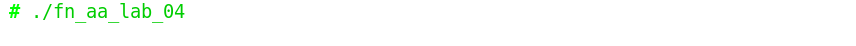
\includegraphics[scale=0.6]{./images/example1.png}
    \caption{Пустой ввод}
    \label{img:ex1}
\end{figure}

\begin{figure}[H]
    \centering
    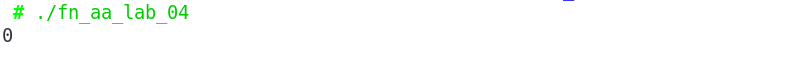
\includegraphics[scale=0.6]{./images/example2.png}
    \caption{Невозможное кол-во потоков}
    \label{img:ex2}
\end{figure}

\begin{figure}[H]
    \centering
    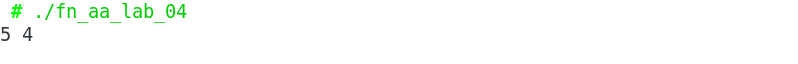
\includegraphics[scale=0.6]{./images/example3.png}
    \caption{Длина матрицы меньше кол-ва потоков}
    \label{img:ex3}
\end{figure}

\begin{figure}[H]
    \centering
    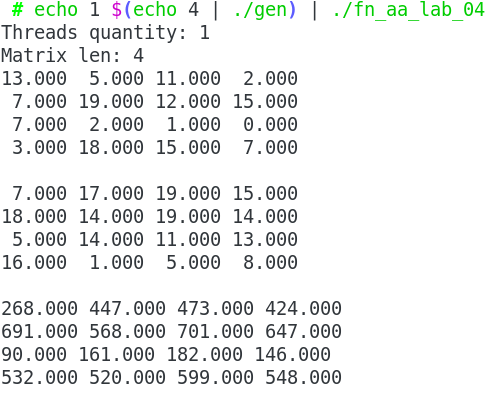
\includegraphics[scale=0.6]{./images/example4.png}
    \caption{Работа одного потока на матрицах длины 4}
    \label{img:ex4}
\end{figure}

\begin{figure}[H]
    \centering
    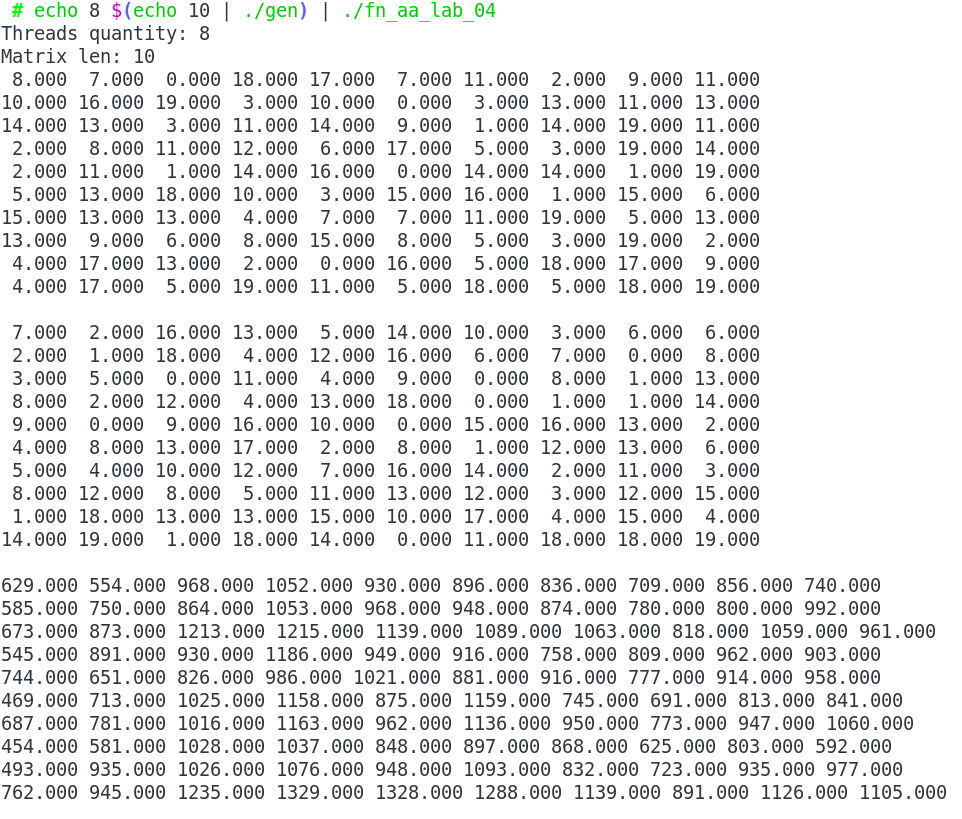
\includegraphics[scale=0.6]{./images/example5.png}
    \caption{Работа восьми потоков на матрицах длины 10}
    \label{img:ex5}
\end{figure}

\section{Описание тестирования}

В таблице \ref{table:test} приведены тестовые данные.

\begin{table}[H]
    \caption{Тестовые данные}
    \label{table:test}
    \centering
    \begin{tabular}{|c|c|c|}
        \hline
        Первая матрица & Вторая матрица & Ожидаемый результат \\
        \hline
        1 2 & 1 2 & \ 7 10 \\
        3 4 & 3 4 & 15 22 \\
        \hline
        1 2 3 & 1 2 3 & \ 30\ \ 36\ \ 42 \\
        4 5 6 & 4 5 6 & \ 66\ \ 81\ \ 96 \\
        7 8 9 & 7 8 9 & 102 126 150 \\
        \hline
        1 0 0 & 1 2 3 & 1 2 3 \\
        0 1 0 & 4 5 6 & 4 5 6 \\
        0 0 1 & 7 8 9 & 7 8 9 \\
        \hline
    \end{tabular}
\end{table}

В таблицах \ref{table:wtest}, \ref{table:pwtest} приведены результаты тестирования. Все тесты были успешно пройдены.

\begin{table}[H]
    \caption{Результаты тестирования алгоритма Винограда}
    \label{table:wtest}
    \centering
    \begin{tabular}{|c|c|c|}
        \hline
        Первая матрица & Вторая матрица & Полученный результат \\
        \hline
        1 2 & 1 2 & \ 7 10 \\
        3 4 & 3 4 & 15 22 \\
        \hline
        1 2 3 & 1 2 3 & \ 30\ \ 36\ \ 42 \\
        4 5 6 & 4 5 6 & \ 66\ \ 81\ \ 96 \\
        7 8 9 & 7 8 9 & 102 126 150 \\
        \hline
        1 0 0 & 1 2 3 & 1 2 3 \\
        0 1 0 & 4 5 6 & 4 5 6 \\
        0 0 1 & 7 8 9 & 7 8 9 \\
        \hline
    \end{tabular}
\end{table}

\begin{table}[H]
    \caption{Результаты тестирования параллелизированного алгоритма Винограда}
    \label{table:pwtest}
    \centering
    \begin{tabular}{|c|c|c|}
        \hline
        Первая матрица & Вторая матрица & Полученный результат \\
        \hline
        1 2 & 1 2 & \ 7 10 \\
        3 4 & 3 4 & 15 22 \\
        \hline
        1 2 3 & 1 2 3 & \ 30\ \ 36\ \ 42 \\
        4 5 6 & 4 5 6 & \ 66\ \ 81\ \ 96 \\
        7 8 9 & 7 8 9 & 102 126 150 \\
        \hline
        1 0 0 & 1 2 3 & 1 2 3 \\
        0 1 0 & 4 5 6 & 4 5 6 \\
        0 0 1 & 7 8 9 & 7 8 9 \\
        \hline
    \end{tabular}
\end{table}

\section{Вывод}
Для реализации программы были выбраны средства разработки: язык программирование C++, библиотеки std::chrono, std::thread, а так же подготовлены тестовые данные и успешно проведено тестирование.

